%%%%%%%%%%%%%%%%%%%%%%%%%%%%%%%%%%%%%%%%%%%%%%%%%%%%%%%%%%%%%%%%%%%%%%
%%  Copyright by Wenliang Du.                                       %%
%%  This work is licensed under the Creative Commons                %%
%%  Attribution-NonCommercial-ShareAlike 4.0 International License. %%
%%  To view a copy of this license, visit                           %%
%%  http://creativecommons.org/licenses/by-nc-sa/4.0/.              %%
%%%%%%%%%%%%%%%%%%%%%%%%%%%%%%%%%%%%%%%%%%%%%%%%%%%%%%%%%%%%%%%%%%%%%%

\documentclass[11pt]{article}

\usepackage[most]{tcolorbox}
\usepackage{times}
\usepackage{epsf}
\usepackage{epsfig}
\usepackage{amsmath, alltt, amssymb, xspace}
\usepackage{wrapfig}
\usepackage{fancyhdr}
\usepackage{url}
\usepackage{verbatim}
\usepackage{fancyvrb}
\usepackage{adjustbox}
\usepackage{listings}
\usepackage{color}
\usepackage{subfigure}
\usepackage{cite}
\usepackage{sidecap}
\usepackage{pifont}
\usepackage{mdframed}
\usepackage{textcomp}
\usepackage{enumitem}


% Horizontal alignment
\topmargin      -0.50in  % distance to headers
\oddsidemargin  0.0in
\evensidemargin 0.0in
\textwidth      6.5in
\textheight     8.9in 

\newcommand{\todo}[1]{
\vspace{0.1in}
\fbox{\parbox{6in}{TODO: #1}}
\vspace{0.1in}
}


\newcommand{\unix}{{\tt Unix}\xspace}
\newcommand{\linux}{{\tt Linux}\xspace}
\newcommand{\minix}{{\tt Minix}\xspace}
\newcommand{\ubuntu}{{\tt Ubuntu}\xspace}
\newcommand{\setuid}{{\tt Set-UID}\xspace}
\newcommand{\openssl} {\texttt{openssl}}


\pagestyle{fancy}
\lhead{\bfseries SEED Labs}
\chead{}
\rhead{\small \thepage}
\lfoot{}
\cfoot{}
\rfoot{}


\definecolor{dkgreen}{rgb}{0,0.6,0}
\definecolor{gray}{rgb}{0.5,0.5,0.5}
\definecolor{mauve}{rgb}{0.58,0,0.82}
\definecolor{lightgray}{gray}{0.90}


\lstset{%
  frame=none,
  language=,
  backgroundcolor=\color{lightgray},
  aboveskip=3mm,
  belowskip=3mm,
  showstringspaces=false,
%  columns=flexible,
  basicstyle={\small\ttfamily},
  numbers=none,
  numberstyle=\tiny\color{gray},
  keywordstyle=\color{blue},
  commentstyle=\color{dkgreen},
  stringstyle=\color{mauve},
  breaklines=true,
  breakatwhitespace=true,
  tabsize=3,
  columns=fullflexible,
  keepspaces=true,
  escapeinside={(*@}{@*)}
}

\newcommand{\newnote}[1]{
\vspace{0.1in}
\noindent
\fbox{\parbox{1.0\textwidth}{\textbf{Note:} #1}}
%\vspace{0.1in}
}


%% Submission
\newcommand{\seedsubmission}{You need to submit a detailed lab report, with screenshots,
to describe what you have done and what you have observed.
You also need to provide explanation
to the observations that are interesting or surprising.
Please also list the important code snippets followed by
explanation. Simply attaching code without any explanation will not
receive credits.}

%% Book
\newcommand{\seedbook}{\textit{Computer \& Internet Security: A Hands-on Approach}, 2nd
Edition, by Wenliang Du. See details at \url{https://www.handsonsecurity.net}.}

%% Videos
\newcommand{\seedisvideo}{\textit{Internet Security: A Hands-on Approach},
by Wenliang Du. See details at \url{https://www.handsonsecurity.net/video.html}.}

\newcommand{\seedcsvideo}{\textit{Computer Security: A Hands-on Approach},
by Wenliang Du. See details at \url{https://www.handsonsecurity.net/video.html}.}

%% Lab Environment
\newcommand{\seedenvironment}{This lab has been tested on our pre-built
Ubuntu 16.04 VM, which can be downloaded from the SEED website. }

\newcommand{\seedenvironmentA}{This lab has been tested on our pre-built
Ubuntu 16.04 VM, which can be downloaded from the SEED website. }

\newcommand{\seedenvironmentB}{This lab has been tested on our pre-built
Ubuntu 20.04 VM, which can be downloaded from the SEED website. }

\newcommand{\seedenvironmentAB}{This lab has been tested on our pre-built
Ubuntu 16.04 and 20.04 VMs, which can be downloaded from the SEED website. }

\newcommand{\nodependency}{Since we use containers to set up the lab environment, 
this lab does not depend too much on our SEED VM. You can do this lab
using other VMs or physical machines. }







\newcommand{\seedlabcopyright}[1]{
\vspace{0.1in}
\fbox{\parbox{6in}{\small Copyright \copyright\ {#1}\ \ by Wenliang Du.\\
      This work is licensed under a Creative Commons
      Attribution-NonCommercial-ShareAlike 4.0 International License.
      If you remix, transform, or build upon the material, 
      this copyright notice must be left intact, or reproduced in a way that is reasonable to
      the medium in which the work is being re-published.}}
\vspace{0.1in}
}





\newcommand{\telnet} {\texttt{telnet}\xspace}

\newcommand{\firewallFigs}{./Figs}
\lhead{\bfseries SEED Labs -- Linux Firewall Exploration Lab}

\begin{document}



\begin{center}
{\LARGE Linux Firewall Exploration Lab}
\end{center}

\seedlabcopyright{2006 - 2016}



% *******************************************
% SECTION
% ******************************************* 
\section{Overview}

The learning objective of this lab is for students to gain the 
insights on how firewalls work 
by playing with firewall software and implement a simplified 
packet filtering firewall.
Firewalls have several types; in this lab, we focus on
\textit{packet filter}.
Packet filters inspect packets, and decide 
whether to drop or forward a packet based on firewall rules. 
Packet filters are usually {\em stateless}; they filter each packet based 
only on the information contained in that packet, without paying 
attention to whether a packet is part of an existing stream of traffic.
Packet filters often use a combination of a packet's source and 
destination address, its protocol, and, for TCP and UDP traffic, 
port numbers. 
%Unlike packet filters, which work at the
%network and transport layers, application firewalls work at 
%the application layer. A widely used application firewall 
%is web proxy, which is primarily used for egress filtering of 
%web traffic.  
In this lab, students will play with 
this type of firewall, and also through the implementation of some 
of the key functionalities, they can understand how 
firewalls work. Moreover, students will learn how to use SSH tunnels to bypass firewalls. 
This lab covers the following topics:

\begin{itemize}[noitemsep]
\item Firewall
\item Netfilter
\item Loadable kernel module
\item Bypassing firewalls using SSH tunnel 
\item How to bypassing firewalls using VPN is covered in a separate lab.
\end{itemize}


\paragraph{Readings and videos.}
Detailed coverage of firewalls can be found in the following:

\begin{itemize}
\item Chapter 17 of the SEED Book, \seedbook
\item Section 9 of the SEED Lecture, \seedisvideo
\end{itemize}


\paragraph{Lab environment.} \seedenvironment



% *******************************************
% SECTION
% ******************************************* 
\section{Lab Tasks}



% -------------------------------------------
% SUBSECTION
% ------------------------------------------- 
\subsection{Task 1: Using Firewall}

\linux has a tool called {\tt iptables}, which is essentially a firewall.
In this task, the objective is to use {\tt iptables} to set up some firewall policies, and 
observe the behaviors of your system after the policies become effective.
You need to set up at least two VMs, one called Machine A, and other called 
Machine B. You run the firewall on your Machine A. Basically, we use 
{\tt iptables} as a personal firewall. Optionally, if you have more VMs, you can 
set up a firewall at your router, so it can protect a network, instead of 
just one single computer. After you set up the two VMs, you should perform
the following tasks: 

\begin{itemize}
\item Prevent A from doing \telnet to Machine B.
\item Prevent B from doing \telnet to Machine A.
\item Prevent A from visiting an external web site. You can choose any web
site that you like to block, but keep in mind, some web servers have multiple
IP addresses. 
\end{itemize}


You can find the manual of {\tt iptables} by typing {\tt "man iptables"} or search it
online. We list some commonly used commands 
in the following:


\begin{lstlisting}
// List all the rules in the filter table
$ sudo iptables -L
$ sudo iptables -L --line-numbers

// Delete all the rules in the filter table
$ sudo iptables -F

// Delete the 2nd rule in the INPUT chain of the filter table 
$ sudo iptables -D INPUT 2

// Drop all the incoming packets that satisfy the <rule>
$ sudo iptables -A INPUT <rule>  -j DROP
\end{lstlisting}
 


% -------------------------------------------
% SUBSECTION
% ------------------------------------------- 
\subsection{Task 2: Implementing a Simple Firewall} 

The firewall you used in the previous task is a packet filtering 
type of firewall. The main part of this type of firewall is the filtering part, 
which inspects each incoming and outgoing packets, and enforces the firewall policies 
set by the administrator. Since the packet 
processing is done within the kernel, the filtering must also be 
done within the kernel. Therefore, it seems that implementing such
a firewall requires us to modify the \linux kernel. In the past, 
this had to be done by modifying and rebuilding 
the kernel. The modern \linux 
operating systems provide several new mechanisms 
to facilitate the manipulation of packets without rebuilding
the kernel image. These two mechanisms are 
\textit{Loadable Kernel Module} ({\tt LKM}) and {\tt Netfilter}.
 

{\tt LKM} allows us to add a new module to the kernel at the runtime. 
This new module enables us to extend the functionalities of the kernel,
without rebuilding the kernel or even rebooting the computer. 
The packet filtering part of a firewall can be implemented 
as an LKM. However, this is not enough. In order for the filtering module to 
block incoming/outgoing packets, the module 
must be inserted into the packet processing path. 
This cannot be easily done in the past before 
the {\tt Netfilter} was introduced into the \linux.


{\tt Netfilter} is designed to facilitate the manipulation of 
packets by authorized users. {\tt Netfilter} achieves this 
goal by implementing a number of {\em hooks} in the 
\linux kernel. These hooks are inserted into various places, 
including the packet incoming and outgoing paths. 
If we want to manipulate the incoming packets, we simply
need to connect our own programs (within LKM) to the 
corresponding hooks. Once an incoming packet arrives, 
our program will be invoked. Our program can decide 
whether this packet should be blocked or not; moreover,
we can also modify the packets in the program.


In this task, you need to use LKM and {\tt Netfilter} to implement
the packet filtering module.  This module will fetch 
the firewall policies from a data structure, and use the 
policies to decide whether packets should be blocked or not.
To make your life easier, so you can focus on the filtering part, 
the core of firewalls, we allow you to hardcode your firewall policies 
in the program. You should support at least five different 
rules, including the ones specified in the previous task. 
Guidelines on how to use \texttt{Netfilter} can be 
found in Section~\ref{firewall:sec:guidelines}. In addition, 
Chapter 14 (\S 14.4) of the SEED book provides more detailed explanation on \texttt{Netfilter}. 


\paragraph{Note for Ubuntu 16.04 VM:}
The code in the SEED book was developed in Ubuntu 12.04. It needs to be changed slightly 
to work in Ubuntu 16.04. The change is in the definition of the 
callback function \texttt{telnetFilter()}, because
the prototype of \texttt{Netfilter}'s callback function has been changed in
Ubuntu 16.04. See the difference in the following:


\begin{lstlisting}
// In Ubuntu 12.04
unsigned int telnetFilter(unsigned int hooknum, struct sk_buff *skb,
           const struct net_device *in, const struct net_device *out,
           int (*okfn)(struct sk_buff *)) 

// In Ubuntu 16.04
unsigned int telnetFilter(void *priv, struct sk_buff *skb,
                          const struct nf_hook_state *state)
\end{lstlisting}
 




% -------------------------------------------
% SUBSECTION
% ------------------------------------------- 
\subsection{Task 3: Evading Egress Filtering}

Many companies and schools enforce egress filtering, which blocks users
inside of their networks from reaching out to certain web sites or Internet
services. They do allow users to access other web sites. 
In many cases, this type of firewalls inspect 
the destination IP address and port number in the outgoing packets. If 
a packet matches the restrictions, it will be dropped. 
They usually do not conduct deep packet inspections (i.e., looking into
the data part of packets) due to the performance reason. 
In this task, we show how such egress filtering can be bypassed using
the tunnel mechanism. There are many ways to establish tunnels; 
in this task, we only focus on SSH tunnels.

You need two VMs A and B for this task (three will be better). Machine A is running 
behind a firewall (i.e., inside the company or school's network), and Machine B 
is outside of the firewall.
Typically, there is a dedicated machine that runs the firewall, but
in this task, for the sake of convenience, you can run the firewall 
on Machine A.
You can use {\tt iptables} to set up the following
two firewall rules:


\begin{itemize}
\item \underline{Block all the outgoing traffic to external telnet servers.}  In
reality, the servers that are blocked are usually game servers or other
types of servers that may affect the productivity of employees. In this 
task, we use the telnet server for demonstration purposes. You can run
the telnet server on Machine B.
If you have a third VM, Machine C, you can run the 
telnet server on Machine C. 


\item \underline{Block all the outgoing traffic to {\tt www.facebook.com},} so employees 
(or school kids) are not distracted during their work/school hours. Social
network sites are commonly blocked by companies and schools. After 
you set up the firewall, launch your Firefox browser, and try to connect to Facebook, and report
what happens. If you have already visited Facebook before using this 
browser, you need to clear all the caches using 
Firefox's menu: 
\texttt{Edit -> Preferences -> Privacy \& Security (left pane) -> Clear History (Button on right)}; 
otherwise, the cached
pages may be displayed. If everything is set up properly, you 
should not be able to see Facebook pages. 
It should be noted that Facebook has many IP addresses, it can 
change over the time. Remember to check whether the address is 
still the same by using {\tt ping} or {\tt dig} command. If 
the address has changed, you need to update your firewall rules. 
You can also choose web sites with static IP addresses, instead of using Facebook.
For example, most universities' web servers use static IP addresses (e.g. 
{\tt www.syr.edu}); for demonstration purposes, 
you can try block these IPs, instead of Facebook. 

\end{itemize}



%--------------------------------
\paragraph{Task 3.a: Telnet to Machine B through the firewall}


\begin{figure}[htb]
\begin{center}
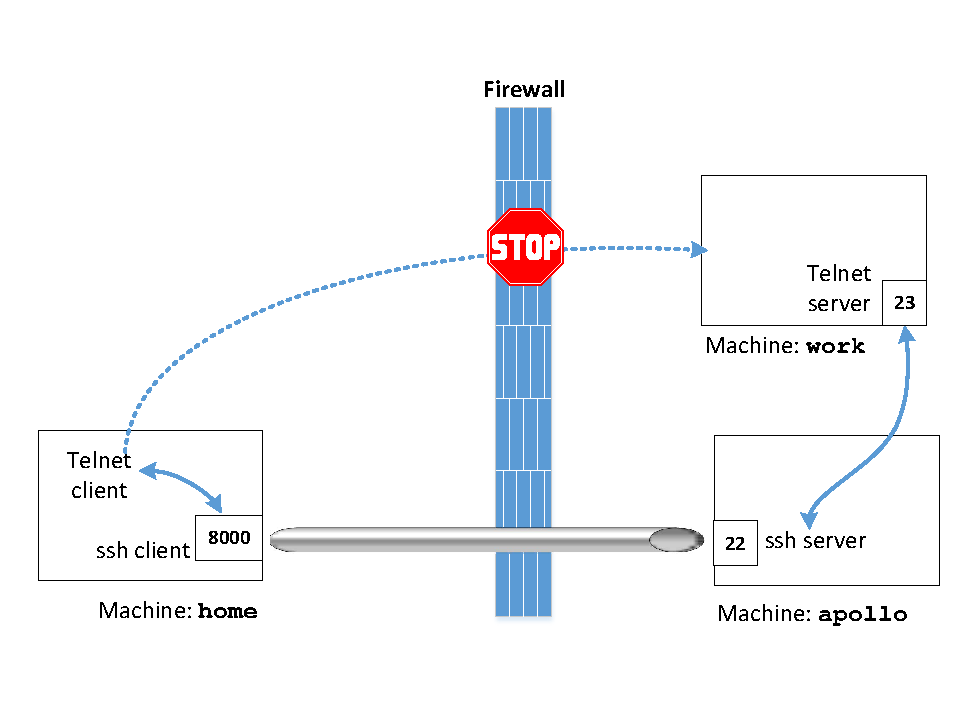
\includegraphics[width=0.7\textwidth]{\firewallFigs/ssh_tunnel.pdf}
\end{center}
\caption{SSH Tunnel Example}
\label{firewall:fig:sshtunnel}
\end{figure}
 

To bypass the firewall, we can establish an SSH tunnel between
Machine A and B, so all the telnet traffic will go through this tunnel
(encrypted), evading the inspection. Figure~\ref{firewall:fig:sshtunnel}
illustrates how the tunnel works. 
The following command 
establishes an SSH tunnel between the localhost (port 8000) and 
machine B (using the default port 22); when packets come out of B's end, it will
be forwarded to Machine C's port 23 (\telnet port). If you only have two VMs,
you can use one VM for both Machine B and Machine C.


\begin{lstlisting}
$ ssh -L 8000:Machine_C_IP:23  seed@Machine_B_IP

// We can now telnet to Machine C via the tunnel:
$ telnet localhost 8000
\end{lstlisting}

When we \telnet to \texttt{localhost}'s port \texttt{8000},  
SSH will transfer all our TCP packets from
one end of the tunnel on \texttt{localhost:8000} to the other end of the tunnel
on Machine B; from there,
the packets will be forwarded to \texttt{Machine\_C:23}. Replies from Machine C will
take a reverse path, and eventually reach our telnet client.
Essentially, we are able to telnet to Machine C.
Please describe your observation and explain how you are able to 
bypass the egress filtering. You should use Wireshark to see
what exactly is happening on the wire.



%--------------------------------
\paragraph{Task 3.b: Connect to Facebook using SSH Tunnel.}
To achieve this goal, we can use the approach similar to that in 
Task 3.a, i.e., establishing a tunnel between your localhost:port
and Machine B, and ask B to forward packets to Facebook. To do 
that, you can use the following command to set up the tunnel:
{\tt "ssh -L 8000:FacebookIP:80 ..."}. 
We will not use this approach, and instead, we 
use a more generic approach, called dynamic port forwarding, instead of a static one
like that in Task 3.a. To do that, we only specify the local
port number, not the final destination. When Machine B receives
a packet from the tunnel, it will dynamically decide where it should 
forward the packet to based on the destination information of
the packet.


\begin{lstlisting}[backgroundcolor=]
$ ssh -D 9000 -C seed@machine_B
\end{lstlisting}


\begin{figure}[htb]
  \begin{center}
     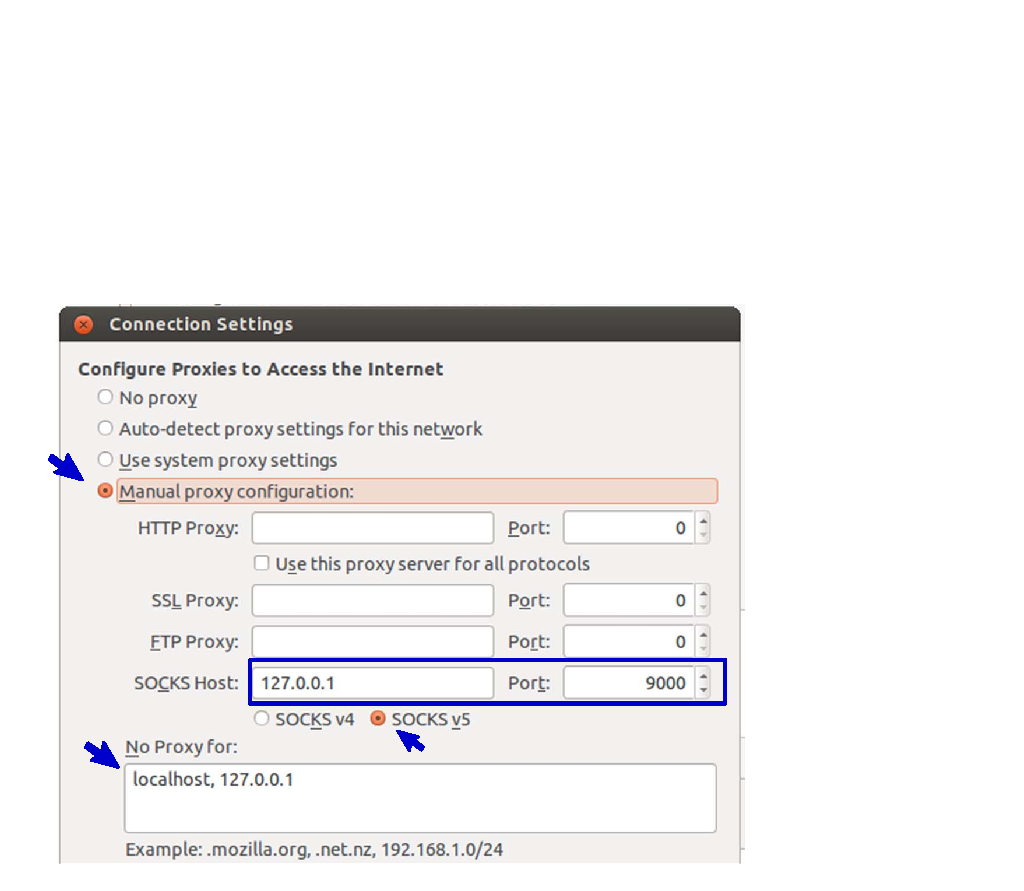
\includegraphics[width=0.8\textwidth]{\firewallFigs/SOCKS_config.pdf}
  \end{center}
  \caption{Configure the SOCKS Proxy}
  \label{firewall:fig:socks_config}
\end{figure}



Similar to the telnet program, which connects {\tt localhost:9000}, 
we need to ask Firefox to connect to {\tt localhost:9000} every time it 
needs to connect to a web server, so the traffic can 
go through our SSH tunnel. To achieve that, we can tell Firefox to
use {\tt localhost:9000} as its proxy. 
To support dynamic port forwarding, we need a special type of proxy 
called \textit{SOCKS proxy}, which is supported by most browsers. 
To set up the proxy in Firefox, go to the menu bar, 
click \texttt{Edit -> Preferences}, 
scroll down to \texttt{Network Proxy},  and
click the \texttt{Settings} button.
Then follow Figure~\ref{firewall:fig:socks_config}.
After the setup is done, please do the following:


\begin{enumerate}
\item Run Firefox and go visit the Facebook page.
Can you see the Facebook page? 
Please describe your observation. 

\item After you get the facebook page, break the SSH tunnel, 
clear the Firefox cache, and try the connection again. 
Please describe your observation. 

\item Establish the SSH tunnel again and connect to Facebook. 
Describe your observation. 

\item Please explain what you have observed, especially
on why the SSH tunnel can help bypass the egress filtering. 
You should use Wireshark to see
what exactly is happening on the wire. Please describe your 
observations and explain them using the packets that you
have captured.
\end{enumerate}


% -------------------------------------------
% SUBSECTION
% ------------------------------------------- 
\subsection{Task 4: Evading Ingress Filtering}


Machine A runs a web server behind a firewall; so only the machines 
in the internal network can access this web server. 
You are working from home and needs to access this internal web server. 
You do not have VPN, but you have SSH, which is considered as 
a poor man's VPN. You do have an account on Machine A (or another internal machine behind the firewall), 
but the firewall also blocks incoming SSH connection, so you cannot SSH into any machine on the
internal network. Otherwise, you can use the same technique from Task 3 to access the web server. 
The firewall, however, does not block outgoing SSH connection, i.e., 
if you want to connect to an outside SSH server, you can still do that. 


The objective of this task is to be able to access the web server on Machine A from
outside.  We will use two machines to emulate the setup. Machine A is the internal computer,
running the protected web server; Machine B is the outside machine at home. 
On Machine A, we block Machine B from accessing its port 80 (web server) and 22 (SSH server).
You need to set up a reverse SSH tunnel on Machine A, so once you get home, you can 
still access the protected web server on A from home. 




% *******************************************
% SECTION
% ******************************************* 
\section{Guidelines}
\label{firewall:sec:guidelines}


\subsection{Loadable Kernel Module}

The following is a simple loadable kernel module. It prints out 
{\tt "Hello World!"} when the module is loaded; when the module
is removed from the kernel, it prints out {\tt "Bye-bye World!"}.
The messages are not printed out on the screen; they are 
actually printed into the {\tt /var/log/syslog} file. You can
use {\tt dmesg | tail -10} to read the last 10 lines of message.


\begin{lstlisting}
#include <linux/module.h>
#include <linux/kernel.h>

int init_module(void)
{
    printk(KERN_INFO "Hello World!\n");
    return 0;
}

void cleanup_module(void)
{
    printk(KERN_INFO "Bye-bye World!.\n");
}
\end{lstlisting}

We now need to create {\tt Makefile}, which includes the following
contents (the above program is named {\tt hello.c}). Then 
just type {\tt make}, and the above program will be compiled
into a loadable kernel module.



\begin{lstlisting}
obj-m += hello.o

all:
        make -C /lib/modules/$(shell uname -r)/build M=$(PWD) modules

clean:
        make -C /lib/modules/$(shell uname -r)/build M=$(PWD) clean
\end{lstlisting}


Once the module is built by typing {\tt make}, you can use the following commands to 
load the module, list all modules, and remove the module:

\begin{lstlisting}
 $ sudo insmod mymod.ko        (inserting a module)
 $ lsmod                       (list all modules)
 $ sudo rmmod mymod.ko         (remove the module)
\end{lstlisting}

Also, you can use {\tt modinfo mymod.ko} to show information about a 
Linux Kernel module.




% -------------------------------------------
% SUBSECTION
% ------------------------------------------- 
\subsection{A Simple Program that Uses Netfilter}

Using {\tt Netfilter} is quite straightforward. All we need to do
is to hook our functions (in the kernel module) to the corresponding
{\tt Netfilter} hooks. Here we show an example:


\begin{lstlisting}
#include <linux/module.h>
#include <linux/kernel.h>
#include <linux/netfilter.h>
#include <linux/netfilter_ipv4.h>


/* This is the structure we shall use to register our function */
static struct nf_hook_ops nfho;

/* This is the hook function itself */
unsigned int hook_func(void *priv, struct sk_buff *skb, 
                       const struct nf_hook_state *state)

{
    /* This is where you can inspect the packet contained in
       the structure pointed by skb, and decide whether to accept 
       or drop it. You can even modify the packet */

    // In this example, we simply drop all packets
    return NF_DROP;           /* Drop ALL packets */
}

/* Initialization routine */
int init_module()
{   /* Fill in our hook structure */
    nfho.hook = hook_func;         /* Handler function */
    nfho.hooknum  = NF_INET_PRE_ROUTING; /* First hook for IPv4 */
    nfho.pf       = PF_INET;
    nfho.priority = NF_IP_PRI_FIRST;   /* Make our function first */

    nf_register_hook(&nfho);
    return 0;
}

/* Cleanup routine */
void cleanup_module()
{
    nf_unregister_hook(&nfho);
}
\end{lstlisting}




% *******************************************
% SECTION
% ******************************************* 
\section{Submission and Demonstration}


\seedsubmission



\end{document}
%%%%%%%%%%%%%%%%%%%%%%%%%%%%%%%%%%%%%%%%%%%%%%%%%%%%%%%%
%%%%%%%%%%%%%%%%%%%%%%%%%%%%%%%%%%%%%%%%%%%%%%%%%%%%%%%%



